%  A simple AAU report template.
%  2015-05-08 v. 1.2.0
%  Copyright 2010-2015 by Jesper Kjær Nielsen <jkn@es.aau.dk>
%
%  This is free software: you can redistribute it and/or modify
%  it under the terms of the GNU General Public License as published by
%  the Free Software Foundation, either version 3 of the License, or
%  (at your option) any later version.
%
%  This is distributed in the hope that it will be useful,
%  but WITHOUT ANY WARRANTY; without even the implied warranty of
%  MERCHANTABILITY or FITNESS FOR A PARTICULAR PURPOSE.  See the
%  GNU General Public License for more details.
%
%  You can find the GNU General Public License at <http://www.gnu.org/licenses/>.
%
%  A simple AAU report template.
%  2015-05-08 v. 1.2.0
%  Copyright 2010-2015 by Jesper Kjær Nielsen <jkn@es.aau.dk>
%
%  This is free software: you can redistribute it and/or modify
%  it under the terms of the GNU General Public License as published by
%  the Free Software Foundation, either version 3 of the License, or
%  (at your option) any later version.
%
%  This is distributed in the hope that it will be useful,
%  but WITHOUT ANY WARRANTY; without even the implied warranty of
%  MERCHANTABILITY or FITNESS FOR A PARTICULAR PURPOSE.  See the
%  GNU General Public License for more details.
%
%  You can find the GNU General Public License at <http://www.gnu.org/licenses/>.
%
\documentclass[11pt,twoside,a4paper,openany]{report}
%%%%%%%%%%%%%%%%%%%%%%%%%%%%%%%%%%%%%%%%%%%%%%%%
% Language, Encoding and Fonts
% http://en.wikibooks.org/wiki/LaTeX/Internationalization
%%%%%%%%%%%%%%%%%%%%%%%%%%%%%%%%%%%%%%%%%%%%%%%%
% Select encoding of your inputs. Depends on
% your operating system and its default input
% encoding. Typically, you should use
%   Linux  : utf8 (most modern Linux distributions)
%            latin1 
%   Windows: ansinew
%            latin1 (works in most cases)
%   Mac    : applemac
% Notice that you can manually change the input
% encoding of your files by selecting "save as"
% an select the desired input encoding. 
\usepackage[utf8]{inputenc}
% Make latex understand and use the typographic
% rules of the language used in the document.
\usepackage[danish,english]{babel}
% hide border around links
\usepackage[hidelinks]{hyperref}
% Use the palatino font
\usepackage[sc]{mathpazo}
\linespread{1.05}         % Palatino needs more leading (space between lines)
% Choose the font encoding
\usepackage[T1]{fontenc}
%%%%%%%%%%%%%%%%%%%%%%%%%%%%%%%%%%%%%%%%%%%%%%%%
% Graphics and Tables
% http://en.wikibooks.org/wiki/LaTeX/Importing_Graphics
% http://en.wikibooks.org/wiki/LaTeX/Tables
% http://en.wikibooks.org/wiki/LaTeX/Colors
%%%%%%%%%%%%%%%%%%%%%%%%%%%%%%%%%%%%%%%%%%%%%%%%
% load a colour package
\usepackage{xcolor}
\definecolor{aaublue}{RGB}{33,26,82}% dark blue
% The standard graphics inclusion package
\usepackage{graphicx}
% Set up how figure and table captions are displayed
\usepackage{caption}
\captionsetup{%
  font=footnotesize,% set font size to footnotesize
  labelfont=bf % bold label (e.g., Figure 3.2) font
}
% Make the standard latex tables look so much better
\usepackage{array,booktabs}
% Enable the use of frames around, e.g., theorems
% The framed package is used in the example environment
\usepackage{framed}

%%%%%%%%%%%%%%%%%%%%%%%%%%%%%%%%%%%%%%%%%%%%%%%%
% Mathematics
% http://en.wikibooks.org/wiki/LaTeX/Mathematics
%%%%%%%%%%%%%%%%%%%%%%%%%%%%%%%%%%%%%%%%%%%%%%%%
% Defines new environments such as equation,
% align and split 
\usepackage{amsmath}
% Adds new math symbols
\usepackage{amssymb}
% Use theorems in your document
% The ntheorem package is also used for the example environment
% When using thmmarks, amsmath must be an option as well. Otherwise \eqref doesn't work anymore.
\usepackage[framed,amsmath,thmmarks]{ntheorem}

%%%%%%%%%%%%%%%%%%%%%%%%%%%%%%%%%%%%%%%%%%%%%%%%
% Page Layout
% http://en.wikibooks.org/wiki/LaTeX/Page_Layout
%%%%%%%%%%%%%%%%%%%%%%%%%%%%%%%%%%%%%%%%%%%%%%%%
% Change margins, papersize, etc of the document
\usepackage[
  inner=28mm,% left margin on an odd page
  outer=41mm,% right margin on an odd page
  ]{geometry}
% Modify how \chapter, \section, etc. look
% The titlesec package is very configureable [display] \chaptertitlename\
\usepackage{titlesec}
\titleformat{\chapter}{\normalfont\huge\bfseries}{ \thechapter}{20pt}{\Huge}
\titleformat*{\section}{\normalfont\Large\bfseries}
\titleformat*{\subsection}{\normalfont\large\bfseries}
\titleformat*{\subsubsection}{\normalfont\normalsize\bfseries}
%\titleformat*{\paragraph}{\normalfont\normalsize\bfseries}
%\titleformat*{\subparagraph}{\normalfont\normalsize\bfseries}

% Clear empty pages between chapters
\let\origdoublepage\cleardoublepage
\newcommand{\clearemptydoublepage}{%
  \clearpage
  {\pagestyle{empty}\origdoublepage}%
}
\let\cleardoublepage\clearemptydoublepage

% Change the headers and footers
\usepackage{fancyhdr}
\pagestyle{fancy}
\fancyhf{} %delete everything
\renewcommand{\headrulewidth}{0pt} %remove the horizontal line in the header
\fancyhead[RE]{\small\nouppercase\leftmark} %even page - chapter title
\fancyhead[LO]{\small\nouppercase\rightmark} %uneven page - section title
\fancyhead[LE,RO]{\thepage} %page number on all pages
% Do not stretch the content of a page. Instead,
% insert white space at the bottom of the page
\raggedbottom
% Enable arithmetics with length. Useful when
% typesetting the layout.
\usepackage{calc}

%%%%%%%%%%%%%%%%%%%%%%%%%%%%%%%%%%%%%%%%%%%%%%%%
% Bibliography
% http://en.wikibooks.org/wiki/LaTeX/Bibliography_Management
%%%%%%%%%%%%%%%%%%%%%%%%%%%%%%%%%%%%%%%%%%%%%%%%
\usepackage[backend=bibtex,
  bibencoding=utf8
  ]{biblatex}
\addbibresource{bib/mybib}

%%%%%%%%%%%%%%%%%%%%%%%%%%%%%%%%%%%%%%%%%%%%%%%%
% Misc
%%%%%%%%%%%%%%%%%%%%%%%%%%%%%%%%%%%%%%%%%%%%%%%%
% Add bibliography and index to the table of
% contents
\usepackage[nottoc]{tocbibind}
% Add the command \pageref{LastPage} which refers to the
% page number of the last page
\usepackage{lastpage}
% Add todo notes in the margin of the document
\usepackage[
%  disable, %turn off todonotes
  colorinlistoftodos, %enable a coloured square in the list of todos
  textwidth=\marginparwidth, %set the width of the todonotes
  textsize=scriptsize, %size of the text in the todonotes
  ]{todonotes}
% For typesetting C codes
\usepackage{listings}
%%%%%%%%%%%%%%%%%%%%%%%%%%%%%%%%%%%%%%%%%%%%%%%%
% Hyperlinks
% http://en.wikibooks.org/wiki/LaTeX/Hyperlinks
%%%%%%%%%%%%%%%%%%%%%%%%%%%%%%%%%%%%%%%%%%%%%%%%
% Enable hyperlinks and insert info into the pdf
% file. Hypperref should be loaded as one of the 
% last packages
\usepackage{hyperref}
\usepackage{xcolor} %custom colours
\usepackage{mdframed} %nice frames

\definecolor{light-gray}{gray}{0.95} %the shade of grey that stack exchange uses
\definecolor{light-blue}{HTML}{2E86C1} 
\renewcommand{\labelitemii}{$\star$}
\hypersetup{%
	pdfpagelabels=true,%
	plainpages=false,%
	pdfauthor={Author(s)},%
	pdftitle={Title},%
	pdfsubject={Subject},%
	bookmarksnumbered=true,%
	colorlinks=false,%
	citecolor=black,%
	filecolor=black,%
	linkcolor=black,% you should probably change this to black before printing
	urlcolor=black,%
	pdfstartview=FitH%
}
% for symb
\usepackage{gensymb}  
\usepackage{float}  % package inclusion and set up of the document
% see, e.g., http://en.wikibooks.org/wiki/LaTeX/Formatting#Hyphenation
% for more information on word hyphenation
\hyphenation{ex-am-ple hy-phen-a-tion short}
\hyphenation{long la-tex}
% 
%  A simple AAU report template.
%  2015-05-08 v. 1.2.0
%  Copyright 2010-2015 by Jesper Kjær Nielsen <jkn@es.aau.dk>
%
%  This is free software: you can redistribute it and/or modify
%  it under the terms of the GNU General Public License as published by
%  the Free Software Foundation, either version 3 of the License, or
%  (at your option) any later version.
%
%  This is distributed in the hope that it will be useful,
%  but WITHOUT ANY WARRANTY; without even the implied warranty of
%  MERCHANTABILITY or FITNESS FOR A PARTICULAR PURPOSE.  See the
%  GNU General Public License for more details.
%
%  You can find the GNU General Public License at <http://www.gnu.org/licenses/>.
%
%
%
% see, e.g., http://en.wikibooks.org/wiki/LaTeX/Customizing_LaTeX#New_commands
% for more information on how to create macros

%%%%%%%%%%%%%%%%%%%%%%%%%%%%%%%%%%%%%%%%%%%%%%%%
% Macros for the titlepage
%%%%%%%%%%%%%%%%%%%%%%%%%%%%%%%%%%%%%%%%%%%%%%%%
%Creates the aau titlepage
\newcommand{\aautitlepage}[3]{%
  {
    %set up various length
    \ifx\titlepageleftcolumnwidth\undefined
      \newlength{\titlepageleftcolumnwidth}
      \newlength{\titlepagerightcolumnwidth}
    \fi
    \setlength{\titlepageleftcolumnwidth}{0.5\textwidth-\tabcolsep}
    \setlength{\titlepagerightcolumnwidth}{\textwidth-2\tabcolsep-\titlepageleftcolumnwidth}
    %create title page
    \thispagestyle{empty}
    \noindent%
    \begin{tabular}{@{}ll@{}}
      \parbox{\titlepageleftcolumnwidth}{
        \iflanguage{danish}{%
          
\includegraphics[width=\titlepageleftcolumnwidth]{figures/aau_logo_da}
        }{%
          
\includegraphics[width=\titlepageleftcolumnwidth]{figures/aau_logo_en}
        }
      } &
      \parbox{\titlepagerightcolumnwidth}{\raggedleft\sf\small
        #2
      }\bigskip\\
       #1 &
      \parbox[t]{\titlepagerightcolumnwidth}{%
      \textbf{Abstract:}\bigskip\par
        \fbox{\parbox{\titlepagerightcolumnwidth-2\fboxsep-2\fboxrule}{%
          #3
        }}
      }\\
    \end{tabular}
    \vfill
    \iflanguage{danish}{%
      \noindent{\footnotesize\emph{Rapportens indhold er frit tilgængeligt, men offentliggørelse (med kildeangivelse) må kun ske efter aftale med forfatterne.}}
    }{%
      \noindent{\footnotesize\emph{The content of this report is freely available, but publication (with reference) may only be pursued due to agreement with the author.}}
    }
    \clearpage
  }
}

%Create english project info
\newcommand{\englishprojectinfo}[8]{%
  \parbox[t]{\titlepageleftcolumnwidth}{
    \textbf{Title:}\\ #1\bigskip\par
    \textbf{Theme:}\\ #2\bigskip\par
    \textbf{Project Period:}\\ #3\bigskip\par
    \textbf{Project Group:}\\ #4\bigskip\par
    \textbf{Participant(s):}\\ #5\bigskip\par
    \textbf{Supervisor(s):}\\ #6\bigskip\par
    \textbf{Copies:} #7\bigskip\par
    \textbf{Page Numbers:} \pageref{LastPage}\bigskip\par
    \textbf{Date of Completion:}\\ #8
  }
}

%Create danish project info
\newcommand{\danishprojectinfo}[8]{%
  \parbox[t]{\titlepageleftcolumnwidth}{
    \textbf{Titel:}\\ #1\bigskip\par
    \textbf{Tema:}\\ #2\bigskip\par
    \textbf{Projektperiode:}\\ #3\bigskip\par
    \textbf{Projektgruppe:}\\ #4\bigskip\par
    \textbf{Deltager(e):}\\ #5\bigskip\par
    \textbf{Vejleder(e):}\\ #6\bigskip\par
    \textbf{Oplagstal:} #7\bigskip\par
    \textbf{Sidetal:} \pageref{LastPage}\bigskip\par
    \textbf{Afleveringsdato:}\\ #8
  }
}

%%%%%%%%%%%%%%%%%%%%%%%%%%%%%%%%%%%%%%%%%%%%%%%%
% An example environment
%%%%%%%%%%%%%%%%%%%%%%%%%%%%%%%%%%%%%%%%%%%%%%%%
\theoremheaderfont{\normalfont\bfseries}
\theorembodyfont{\normalfont}
\theoremstyle{break}
\def\theoremframecommand{{\color{gray!50}\vrule width 5pt \hspace{5pt}}}
\newshadedtheorem{exa}{Example}[chapter]
\newenvironment{example}[1]{%
		\begin{exa}[#1]
}{%
		\end{exa}
}
% my new macros

\begin{document}
%frontmatter
\pagestyle{empty} %disable headers and footers
\pagenumbering{roman} %use roman page numbering in the frontmatter
%  A simple AAU report template.
%  2015-05-08 v. 1.2.0
%  Copyright 2010-2015 by Jesper Kjær Nielsen <jkn@es.aau.dk>
%
%  This is free software: you can redistribute it and/or modify
%  it under the terms of the GNU General Public License as published by
%  the Free Software Foundation, either version 3 of the License, or
%  (at your option) any later version.
%
%  This is distributed in the hope that it will be useful,
%  but WITHOUT ANY WARRANTY; without even the implied warranty of
%  MERCHANTABILITY or FITNESS FOR A PARTICULAR PURPOSE.  See the
%  GNU General Public License for more details.
%
%  You can find the GNU General Public License at <http://www.gnu.org/licenses/>.
%
\pdfbookmark[0]{Front page}{label:frontpage}%
\begin{titlepage}
  \addtolength{\hoffset}{0.5\evensidemargin-0.5\oddsidemargin} %set equal margins on the frontpage - remove this line if you want default margins
  \noindent%
  \begin{tabular}{@{}p{\textwidth}@{}}
    \toprule[2pt]
    \midrule
    \vspace{0.2cm}
    \begin{center}
    \Huge{\textbf{
      Report Title% insert your title here
    }}
    \end{center}
    \begin{center}
      \Large{
        - Subtitle -% insert your subtitle here
      }
    \end{center}
    \vspace{0.2cm}\\
    \midrule
    \toprule[2pt]
  \end{tabular}
  \vspace{4 cm}
  \begin{center}
    {\large
      Project Report%Insert document type (e.g., Project Report)
    }\\
    \vspace{0.2cm}
    {\Large
      Group Name/Number%Insert your group name or real names here
    }
  \end{center}
  \vfill
  \begin{center}
  Aalborg University\\
  Electronics and IT
  \end{center}
\end{titlepage}
\clearpage

\thispagestyle{empty}
{\small
\strut\vfill % push the content to the bottom of the page
\noindent Copyright \copyright{} Aalborg University 2015\par
\vspace{0.2cm}
\noindent Here you can write something about which tools and software you have used for typesetting the document, running simulations and creating figures. If you do not know what to write, either leave this page blank or have a look at the colophon in some of your books.
}
\clearpage


\pdfbookmark[0]{English title page}{label:titlepage_en}
\aautitlepage{%
  \englishprojectinfo{
    Project Title %title
  }{%
    Scientific Theme %theme
  }{%
    Fall Semester 2010 %project period
  }{%
    XXX % project group
  }{%
    %list of group members
    Author 1\\ 
    Author 2\\
    Author 3
  }{%
    %list of supervisors
    Supervisor 1\\
    Supervisor 2
  }{%
    1 % number of printed copies
  }{%
    \today % date of completion
  }%
}{%department and address
  \textbf{Electronics and IT}\\
  Aalborg University\\
  \href{http://www.aau.dk}{http://www.aau.dk}
}{% the abstract
  Here is the abstract
}

\cleardoublepage
\cleardoublepage
\pdfbookmark[0]{Contents}{label:contents}
\pagestyle{fancy} %enable headers and footers again
\tableofcontents
%\listoftodos
%\chapter*{Preface\markboth{Preface}{Preface}}\label{ch:preface}
\addcontentsline{toc}{chapter}{Preface}
Here is the preface. You should put your signatures at the end of the preface.

\vspace{\baselineskip}\hfill Aalborg University, \today
\vfill\noindent
\begin{minipage}[b]{0.45\textwidth}
 \centering
 \rule{\textwidth}{0.5pt}\\
  Author 1\\
 {\footnotesize <username1@XX.aau.dk>}
\end{minipage}
\hfill
\begin{minipage}[b]{0.45\textwidth}
 \centering
 \rule{\textwidth}{0.5pt}\\
  Author 2\\
 {\footnotesize <username2@XX.aau.dk>}
\end{minipage}
\vspace{3\baselineskip}
\begin{center}
\begin{minipage}[b]{0.45\textwidth}
 \centering
 \rule{\textwidth}{0.5pt}
  Author 3\\
 {\footnotesize <username3@XX.aau.dk>}
\end{minipage}
\end{center}

%\cleardoublepage
%mainmatter
\pagenumbering{arabic} %use arabic page numbering in the mainmatter
\chapter{Introduction}
\section{SECTION NAME}
\subsection{SUBSECTION NAME 1}
\paragraph{}WRITE HERE

\begin{figure}[H]
  \centering
    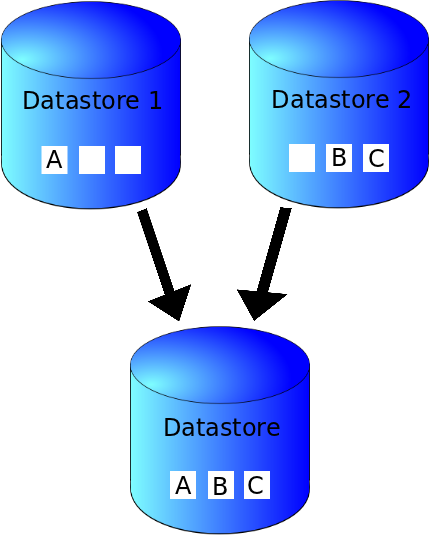
\includegraphics[height= 10cm, width=15cm]{project/images/data-sync}
  \caption{\textbf{IMAGE CAPTION}}
\end{figure}

\subsection{SUBSECTION NAME 2}
\paragraph{}WRITE HERE

\chapter{Development and Simulation}\label{ch:ch2label}
\section{Arduino IDE}
The code to be burnt to the program memory of an \arduino{} is written and compiled in the \emph{Arduino IDE}. The IDE also has a serial monitor, which displays values being recieved in real-time from the Arduino via serial communication through the serial port (COM ports). The IDE verifies for correct C/C++ syntax and compiles it, before linking it to Arduino Library files. This creates the \textit{hex} file that contains the code in binary form. It can either be uploaded to the board directly, which the IDE does with the help of the Bootloader program pre-installed on the Arduino, or it can be fed to a \emph{simulator}, which would simulate and show how the circuit would run and its associated parameters.
\begin{figure}[H]
	\vfill
	\centering
	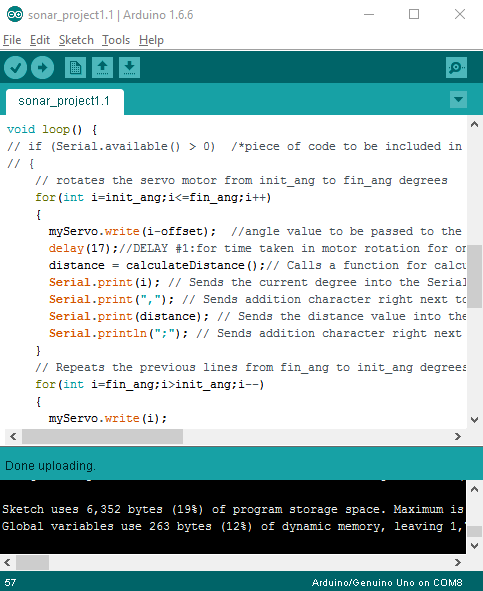
\includegraphics[width=0.5\textwidth]{../Files/IDE}
	\caption{The Arduino IDE}  \label{fig:IDE}
\end{figure}

%\cite{Madsen2010}, \cite{Oetiker2010} and \cite{Mittelbach2005}.

\clearpage

\chapter{Conclusion}

<Conclusion here>

\printbibliography[heading=bibintoc]
\label{bib:mybiblio}
\appendix
\chapter{Appendix A : \arduino{} Code}\label{ch:appAlabel}
Here is the code uploaded on to the \arduinouno{}:
\begin{mdframed}[backgroundcolor=light-gray, roundcorner=10pt,leftmargin=1, rightmargin=1, innerleftmargin=15, innertopmargin=15,innerbottommargin=15, outerlinewidth=1, linecolor=light-gray]
\begin{lstlisting}[caption={The Arduino Code},language = C]
/*ver 1.1 (Final)*/

// Includes the Servo library
#include <Servo.h>. 

// Defines Trig and Echo pins of the Ultrasonic Sensor
const int trigPin = 2;
const int echoPin = 4;

// Variables for the duration & distance measured from the sensor
float duration;
float distance;

//Angle offset between graph and motor's XY axes
int offset = 0;
//Initial and final angles of motor's rotation
//Note that the motor can only take values 0-180.
//Make sure init_angle-offset >=60 to avoid jumper wire obstruction.
int init_ang = 70+offset;
int fin_ang = 180+offset;

// Declares a structure variable/object of the type Servo,
//(defined in the servo library) for controlling the servo motor.
Servo myServo; 

void setup() {
pinMode(trigPin, OUTPUT); // Sets the trigPin as an Output
pinMode(echoPin, INPUT); // Sets the echoPin as an Input
Serial.begin(9600); //Sets baud rate of serial communication
myServo.attach(9); // Defines on which pin is the servo motor attached
}

void loop() {
// if (Serial.available() > 0)  /*piece of code to be included in case of serial communication with IoT board*/
// {
// rotates the servo motor from init_ang to fin_ang degrees
for(int i=init_ang;i<=fin_ang;i++)
{  
myServo.write(i-offset);  //angle value to be passed to the servo library object for writing into the motor
delay(17);//DELAY #1:for time taken in motor rotation for one degree before calculating distance
distance = calculateDistance();// Calls a function for calculating the distance measured by the Ultrasonic sensor for each degree
Serial.print(i); // Sends the current degree into the Serial Port for graphical representation
Serial.print(","); // Sends addition character right next to the previous value needed later in the Processing IDE for indexing
Serial.print(distance); // Sends the distance value into the Serial Port for the graph
Serial.print(";"); // Sends addition character right next to the previous value needed later in the Processing IDE for indexing
}
// Repeats the previous lines from fin_ang to init_ang degrees
for(int i=fin_ang;i>init_ang;i--)
{  
myServo.write(i);
delay(17);  //DELAY #1 //can be minimised to 17 or 1667 microsec
distance = calculateDistance();
Serial.print(i);
Serial.print(",");
Serial.print(distance);
Serial.print(";");
}
//}
}
// Function for calculating the distance measured by the Ultrasonic sensor
float calculateDistance(){ 
unsigned long T1 = micros();
digitalWrite(trigPin, LOW); // trigPin needs a fresh LOW pulse before sending a HIGH pulse that can be detected from echoPin
delayMicroseconds(2);//DELAY #2:time for which low trig pulse is maintained before making it high
digitalWrite(trigPin, HIGH); 
delayMicroseconds(10);//DELAY #3:Sets the trigPin on HIGH state for 10 micro seconds
digitalWrite(trigPin, LOW);
duration = pulseIn(echoPin, HIGH); // Reads the echoPin, returns the sound wave travel time in microseconds
//distance= duration*0.034/2;
distance = (duration/2)/29.1;     //in cm,  datasheet gives "duration/58" as the formula

//To avoid sending data at variable time intervals due to varying time duration taken between execution of above code inside this function depending on distance of obstacle
//if no object, echo pulse is 38ms long HIGH
while(micros()-T1<38000)
{
;
}

return distance;
}
\end{lstlisting}

\end{mdframed}
\clearpage

\chapter{Appendix B : \processing{} Code}\label{ch:appAlabel}
The \emph{Java} code that we ran in \processing{} is given below :
\begin{mdframed}[backgroundcolor=light-gray, roundcorner=10pt,leftmargin=1, rightmargin=1, innerleftmargin=15, innertopmargin=15,innerbottommargin=15, outerlinewidth=1, linecolor=light-gray]
\begin{lstlisting}[caption={The Processing Code}, language=Java]
/*   Arduino Radar Project
*    1.1 [Final and complete]
*   Initialise every variable to null value to avoid null pointer exception
*/

import processing.serial.*; // imports library for serial communication
import java.awt.event.KeyEvent; // imports library for reading the data from the serial port
import java.io.IOException;

Serial myPort; // defines Object Serial
// defines variables
String angle="";
String distance="";
String data="";
String noObject="";
float pixsDistance=0.0;
int iAngle=0;
float iDistance=0.0;
int index1=0;
int index2=0;
int objCount=0,obctr=0;
PFont orcFont;
float angFlag=1.0;
float prevAng=0.0,deltaAng=0.0;
float maxDIST=50.0; //max distance of object in cms
int wctr=0;
float objWidth=0.0,prevWidth=0.0;
void setup() {

size (600, 700); // ***CHANGE THIS TO YOUR SCREEN RESOLUTION***
smooth();

myPort = new Serial(this,"/dev/ttyACM0", 9600); // Enter the COM Port address as COM4 or COM 22.starts the serial communication

myPort.bufferUntil('.'); // reads the data from the serial port up to the character '.'. So actually it reads this: angle,distance.
orcFont = loadFont("CenturySchL-Ital-20.vlw");

}

void draw() {

fill(237,13,245);
textFont(orcFont);
// simulating motion blur and slow fade of the moving line
noStroke();
fill(184,13); 
rect(0, 0, width, height-height*0.065); 

fill(211,27,228); //  color
// calls the functions for drawing the radar
drawRadar(); 
drawLine();
drawObject();
drawText();
}

void serialEvent (Serial myPort) { // starts reading data from the Serial Port
// reads the data from the Serial Port up to the character '.' and puts it into the String variable "data".
try{
data = myPort.readStringUntil(';');
data = data.substring(0,data.length()-1);

index1 = data.indexOf(","); // find the character ',' and puts it into the variable "index1"
angle= data.substring(0, index1); // read the data from position "0" to position of the variable index1 or thats the value of the angle the Arduino Board sent into the Serial Port
distance= data.substring(index1+1, data.length()); // read the data from position "index1" to the end of the data pr thats the value of the distance

// converts the String variables into Integer
iAngle = int(angle);
iDistance = float(distance);
deltaAng=iAngle-prevAng;

if(deltaAng*angFlag<0.0){
objCount=0;
objWidth=0;
}
//anticlockwise--deltaAng>0
//clockwise--deltaAng<0    
if(deltaAng>0.0)
angFlag=1.0;
else
angFlag=-1.0;
}
catch(Exception e){
println("Error parsing:");
e.printStackTrace();
}
}

void drawRadar() {
pushMatrix();
translate(width/2,height-height*0.507); // moves the starting coordinates to new location
noFill();
strokeWeight(2);
stroke(407,409,305);
// draws the arc lines
arc(0,0,(width-width*0.0385),(width-width*0.0385),PI,TWO_PI);
arc(0,0,(width-width*0.26),(width-width*0.26),PI,TWO_PI);
arc(0,0,(width-width*0.498),(width-width*0.498),PI,TWO_PI);
arc(0,0,(width-width*0.754),(width-width*0.754),PI,TWO_PI);
arc(0,0,(width-width*0.0385),(width-width*0.0385),0,PI);
arc(0,0,(width-width*0.26),(width-width*0.26),0,PI);
arc(0,0,(width-width*0.498),(width-width*0.498),0,PI);
arc(0,0,(width-width*0.754),(width-width*0.754),0,PI);
// draws the angle lines
line(-width/2,0,width/2,0);
line(0,0,(-width/2)*cos(radians(30)),(-width/2)*sin(radians(30)));
line(0,0,(-width/2)*cos(radians(60)),(-width/2)*sin(radians(60)));
line(0,0,(-width/2)*cos(radians(90)),(-width/2)*sin(radians(90)));
line(0,0,(-width/2)*cos(radians(120)),(-width/2)*sin(radians(120)));
line(0,0,(-width/2)*cos(radians(150)),(-width/2)*sin(radians(150)));
line(0,0,(-width/2)*cos(radians(180)),(-width/2)*sin(radians(180)));
line(0,0,(-width/2)*cos(radians(210)),(-width/2)*sin(radians(210)));
line(0,0,(-width/2)*cos(radians(240)),(-width/2)*sin(radians(240)));
line(0,0,(-width/2)*cos(radians(270)),(-width/2)*sin(radians(270)));
line(0,0,(-width/2)*cos(radians(300)),(-width/2)*sin(radians(300)));
line(0,0,(-width/2)*cos(radians(330)),(-width/2)*sin(radians(330)));
line((-width/2)*cos(radians(30)),0,width/2,0);
popMatrix();
}

void drawLine() {
pushMatrix();
strokeWeight(8);
stroke(32,65,174); //color for blue line
translate(width/2,height-height*0.507); // moves the starting coordinates to new location
line(0,0,(height-height*0.575)*cos(radians(iAngle)),-(height-height*0.575)*sin(radians(iAngle))); // draws the line according to the angle
popMatrix();
}

void drawObject() {
pushMatrix();
translate(width/2,height-height*0.508); // moves the starting coordinats to new location
strokeWeight(8);
stroke(240,1,40); // red color
pixsDistance = iDistance*((height-height*0.1666)*0.013/3); // covers the distance from the sensor from cm to pixels
if(iDistance<=maxDIST){
if(wctr>2){    //Assuming that an object will be thick enough to be detected for 2 degrees of rotation.
objWidth=0.0;
// draws the object according to the angle and the distance
line(pixsDistance*cos(radians(iAngle)),-pixsDistance*sin(radians(iAngle)),(width-width*0.505)*cos(radians(iAngle)),-(width-width*0.505)*sin(radians(iAngle)));
obctr++;
}
}
popMatrix();
}

void drawText() { // draws the texts on the screen
pushMatrix();
if(iDistance>maxDIST) {
noObject = "No object within Range";
if(wctr==0)
objWidth=prevWidth;
else
objWidth=float(wctr)*iDistance*0.0174;  //width of object in cm
prevWidth=objWidth;
wctr=0;
if(obctr>0){
objCount++;
obctr=0;
}
}
else {
wctr++;
if(wctr>2)  //Assuming that an object will be thick enough to be detected for 2 degrees of rotation.
{
noObject = "Object in Range";

}
} 

fill(0,0,0);  //black background of bottom text
noStroke();
rect(0, height-height*0.0521, width, height);
fill(251,255,249);
textSize(15);

text("30cm",width-width*0.4041,height-height*0.4793);
text("60cm",width-width*0.281,height-height*0.4792);
text("90cm",width-width*0.177,height-height*0.4792);
text("120cm",width-width*0.0729,height-height*0.4792);
textSize(16);
text(noObject, width-width*0.634, height-height*0.0218);
text("Angle: " + iAngle +" @\degree@", width-width*0.97, height-height*0.0232);
text("Distance: ", width-width*0.26, height-height*0.0235);
textSize(16);
text(" No. of objects: "+ objCount +"", width-width*0.986, height-height*0.0714);
text(" Object Width: "+ objWidth +"", width-width*0.986, height-height*0.1714);
if(iDistance<=maxDIST) {
if(wctr>2)
text("        " + iDistance + " cm", width-width*0.185, height-height*0.0237);
}
textSize(19);
fill(7,7,6); //color for degrees text
translate((width-width*0.5020)+width/2*cos(radians(30)),(height-height*0.5283)-width/2*sin(radians(30)));
rotate(-radians(-60));
text("30@\degree@",0,0);
resetMatrix();
translate((width-width*0.507)+width/2*cos(radians(60)),(height-height*0.5139)-width/2*sin(radians(60)));
rotate(-radians(-29));
text("60@\degree@",-4,-5);
resetMatrix();
translate((width-width*0.507)+width/2*cos(radians(90)),(height-height*0.5149)-width/2*sin(radians(90)));
rotate(radians(0));
text("90@@\degree@@",-5,-2);
resetMatrix();
translate(width-width*0.513+width/2*cos(radians(120)),(height-height*0.51286)-width/2*sin(radians(120)));
rotate(radians(-30));
text("120@\degree@",0,0);
resetMatrix();
translate((width-width*0.5298)+width/2*cos(radians(150)),(height-height*0.4803)-width/2*sin(radians(150)));
rotate(radians(-60));
text("150@\degree@",0,0);
resetMatrix();
translate(width-width*0.475+width/2*cos(radians(180)),(height-height*0.47791)-width/2*sin(radians(180)));
rotate(radians(-90));
text("180@\degree@",0,0);
resetMatrix();
translate(width-width*0.494+width/2*cos(radians(210)),(height-height*0.4797)-width/2*sin(radians(210)));
rotate(radians(-120));
text("210@\degree@",0,0);
resetMatrix();
translate(width-width*0.484+width/2*cos(radians(240)),(height-height*0.4867)-width/2*sin(radians(240)));
rotate(radians(-150));
text("240@\degree@",0,0);
resetMatrix();
translate(width-width*0.474+width/2*cos(radians(270)),(height-height*0.50151)-width/2*sin(radians(270)));
rotate(radians(-180));
text("270@\degree@",0,0);
resetMatrix();
translate(width-width*0.470+width/2*cos(radians(300)),(height-height*0.51167)-width/2*sin(radians(300)));
rotate(radians(-210));
text("300@\degree@",0,0);
resetMatrix();
translate(width-width*0.478+width/2*cos(radians(330)),(height-height*0.5174)-width/2*sin(radians(330)));
rotate(radians(-240));
text("330@\degree@",0,0);
resetMatrix();
translate(width-width*0.523+width/2*cos(radians(360)),(height-height*0.52132)-width/2*sin(radians(360)));
rotate(radians(-270));
text("0@\degree@",0,0);
popMatrix(); 
prevAng = iAngle;
}
\end{lstlisting}
\end{mdframed}
\clearpage
\end{document}
